\documentclass[2pt]{scrartcl}
%\documentclass[8pt,landscape]{article}
\usepackage{multicol}
\usepackage{calc}
\usepackage{ifthen}
\usepackage[landscape]{geometry}
\usepackage{amsmath,amsthm,amsfonts,amssymb}
\usepackage{color,graphicx,overpic}
%\usepackage{hyperref}
\usepackage{enumitem}
\newcommand\solution{\textbf{Solution.}}
\setlist{nolistsep}


\pdfinfo{
  /Title (EECS376ExamIStudyGuide.pdf)
  /Creator (TeX)
  /Producer (pdfTeX 1.40.0)
  /Author (Jason R. Berlinsky)
/Keywords (pdflatex, latex,pdftex,tex)}

\ifthenelse{\lengthtest { \paperwidth = 11in}}
{ \geometry{top=.05in,left=.1in,right=.1in,bottom=.05in} }
{\ifthenelse{ \lengthtest{ \paperwidth = 297mm}}
  {\geometry{top=1cm,left=1cm,right=1cm,bottom=1cm} }
  {\geometry{top=0.25cm,left=0.25cm,right=0.25cm,bottom=0.51cm} }
}

\pagestyle{empty}

\makeatletter
\renewcommand{\section}{\@startsection{section}{1}{0mm}
  {-1ex plus -.5ex minus -.2ex}
  {0.5ex plus .2ex}
{\normalfont\large\bfseries}}
\renewcommand{\subsection}{\@startsection{subsection}{2}{0mm}
  {-1explus -.5ex minus -.2ex}
  {0.5ex plus .2ex}
{\normalfont\normalsize\bfseries}}
\renewcommand{\subsubsection}{\@startsection{subsubsection}{3}{0mm}
  {-1ex plus -.5ex minus -.2ex}
  {1ex plus .2ex}
{\normalfont\small\bfseries}}
\makeatother

\def\BibTeX{{\rm B\kern-.05em{\sc i\kern-.025em b}\kern-.08em
T\kern-.1667em\lower.7ex\hbox{E}\kern-.125emX}}

\setcounter{secnumdepth}{0}


\setlength{\parindent}{0pt}
\setlength{\parskip}{0pt plus 0.01ex}

\newtheorem{example}[section]{Example}
% -----------------------------------------------------------------------

\begin{document}

\raggedright
\footnotesize
{\bf NOTE: Please do not delete information from before the midterm. If you want your own copy of a certain size, please make your own file.}

{\bf Contributors: Jason Berlinsky (with credits to study guide contributors)}

{\bf NOTE: This guide IS too long. It will be reduced when all the TODOs are filled in.}
\begin{multicols}{6}


% multicol parameters
% These lengths are set only within the two main columns
%\setlength{\columnseprule}{0.25pt}
  \setlength{\premulticols}{1pt}
  \setlength{\postmulticols}{1pt}
  \setlength{\multicolsep}{1pt}
  \setlength{\columnsep}{1pt}

  \section{Equivalence Relations}
  $R$ is {\bf reflexive} if for every $x$, $xRx$\\
  $R$ is {\bf symmetric} if for every $x$ and $y$, $xRy$ implies $yRx$\\
  $R$ is {\bf transitive} if for every $x, y, z$, $xRy \wedge yRz \rightarrow xRz$
  \section{Boolean Logic}
  $\neg$ - Not\\
  $\wedge$ - And\\
  $\vee$ - Or\\
  $P \wedge (Q \vee R) = (P \wedge Q) \vee (P \wedge R)$\\
  $P \vee (Q \wedge R) = (P \vee Q) \wedge (P \vee R)$\\
  For any two sets $A$ and $B$, $\bar{A \cup B} = \bar{A} \cap \bar{B}$
  \section{Finite Automata}

  \subsection{DFA}

  \begin{multicols}{2}

    Each state must have exactly one transition arrow for every item in the alphabet, and it may only occupy a single state at a time. Formally described by $(Q, \Sigma, \delta, q_0, F)$, where $Q$ is a finite set of states (as $\{q_0, q_1, q_2\}$), $\Sigma$ is the alphabet, $\delta$ is the transition function with domain $Q x \Sigma$ and range $Q$ ($Q x \Sigma \rightarrow Q$), $q_0$ is the start state $\in Q$, and $F$ is the set of accept states, which may be the empty set, $\subset Q$.

    \begin{center}
      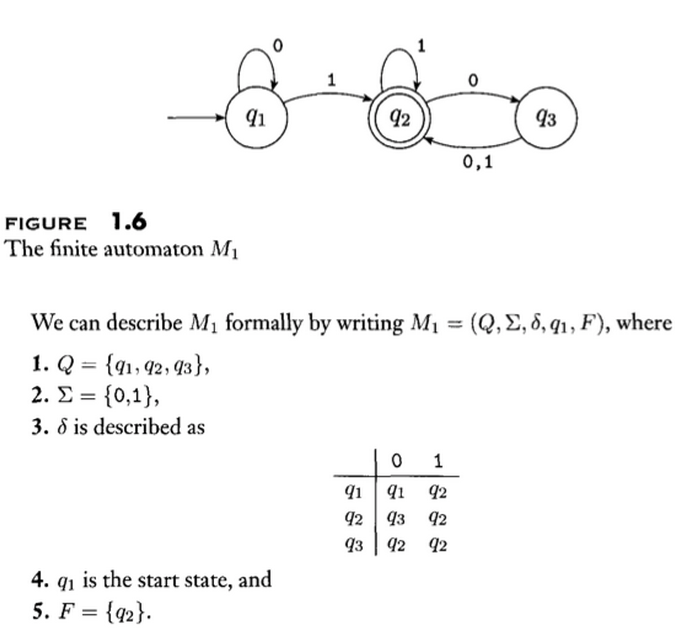
\includegraphics[scale=0.25]{dfa_sample.png}
    \end{center}

  \end{multicols}

  \subsubsection{Complementation}

  Flip acceptance states to get the complement.

  \subsubsection{Combining}

  Let's say there are two DFAs, $A = (Q_1, \Sigma, \delta_1, q_1, F_1)$ and $B = (Q_2, \Sigma, \delta_2, q_2, F_2)$. Let the intersection of the two, $C = (Q_1 \times Q_2, \Sigma, \delta_3, (q_1, q_2), F_1 \times F_2)$, where $\delta_3((r_1, r_2), a) = (\delta_1(r_1, a), \delta_2(r_2, a))$. The union of the two is given by closure properties:
  $A \cup B = \overline{\bar{A} \cap \bar{B}}. F_3 = \overline{\bar{F_1} \times \bar{F_2}}$ 

  \subsection{Regular Operations}

  Union ($\cup$): Returns a set containing all elements that appear in either set.\\
  Concatenation ($.$): Returns a set containing all combinations of an element from set $A$ and an element from set $B$\\
  Star ($*$): Returns a set containing all permutations of each element in a given language. This returns an infinite set. Also all words over the alphabet.

%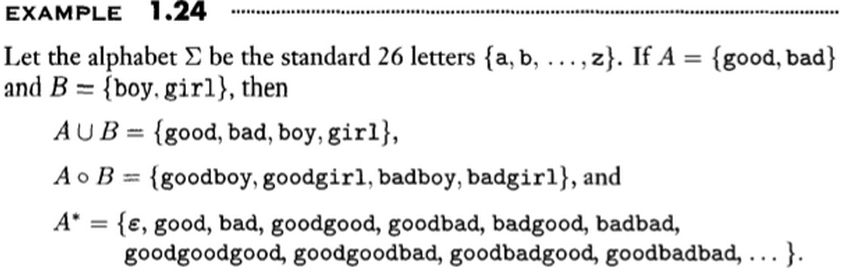
\includegraphics[scale=0.35]{operations.png}

  \subsection{Non-Deterministic}

  A more generalized form of a DFA. Each state does not need a transition arrow for each element in the alphabet. May have more than one active state, may also have more than one transition arrow for a given element in the alphabet. Have a special symbol $\epsilon$ which is followed when present as a transition and does not ``eat" a character from the string.

  Try all legal transitions in parallel. On choice, pick/guess best transition towards acceptance. Accept if there is some path from start to accept.

  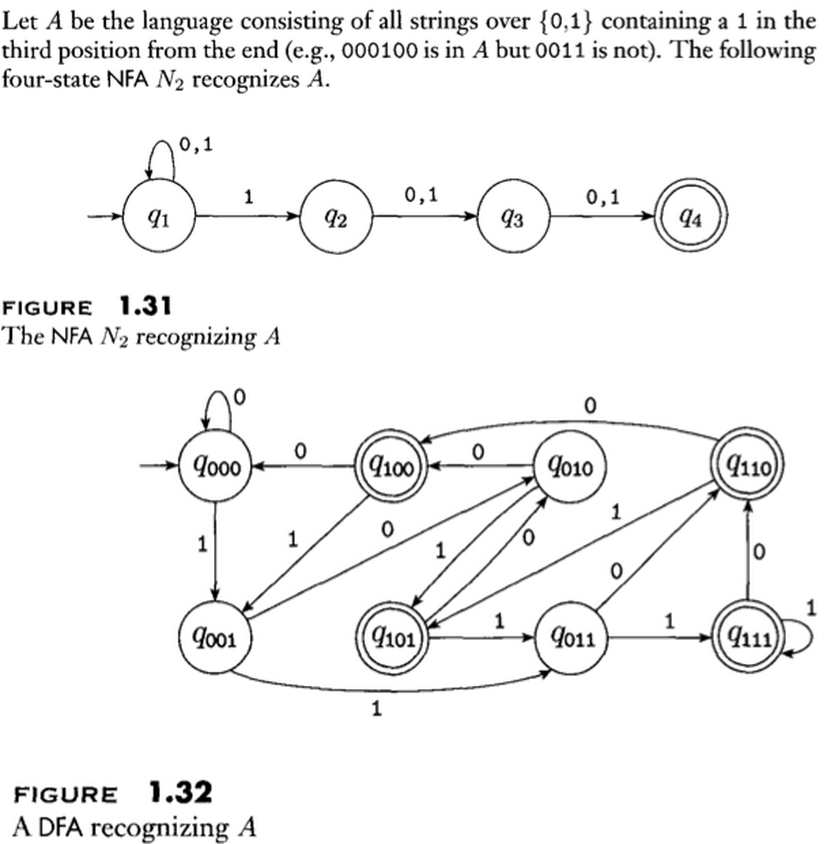
\includegraphics[scale=0.25]{nfa_dfa.png}

  \section{Closure and Projection}

  {\bf Closure:} The idea that any of the regular operations performed on two regular languages will result in another regular language.

  {\bf Projection:} The intersection where all elements in both sets will be present in the new set.

  \section{Regular Expressions}

  Formal definition ($R_n$ are regexps):
  \begin{multicols}{2}
    \begin{itemize}
      \item $\alpha$ for some $a$ in the alphabet $\Sigma$
      \item $\epsilon$
      \item $\emptyset$
      \item $(R_1 \cup R_2)$
      \item $(R_1 . R_2)$
      \item $(R_1^*)$
    \end{itemize}
  \end{multicols}

  $\alpha$ and $\epsilon$ represent the languages $\{\alpha\}, \{\epsilon\}$ respectively, and $\emptyset$ is the empty language. The remaining show what happens when a closure property is applied on the base languages.

  Symbols:
  \begin{itemize}
    \item $\Sigma$: Any symbol in the alphabet
    \item $*$: Repeat the previous character $0$ or more times
    \item $+$: Repeat the previous character $1$ or more times.
  \end{itemize}
  Definitions:
  \begin{multicols}{2}
    \begin{itemize}
      \item $R \cup \emptyset = R$ - Adding the empty language to any other language will not change it
      \item $R . \epsilon = R$ - Joining the empty string to any other string is the same string
      \item $A^* = \{\epsilon\} \cup A \cup AA \cup AAA \cup ...$
      \item $|A \cup B| <= |A| + |B|$
      \item $|AB| <= |A| . |A|$
      \item $\emptyset^* = \{\epsilon\}$. If $A \neq \emptyset$, then $A^*$ is infinite
      \item $L(\underline{\emptyset}) = \emptyset$
      \item $L(\underline{\epsilon}) = \{\epsilon\}$
      \item $L((a \cup b)\epsilon) = \{a, b\}$
      \item $L((a \cup b)\emptyset) = \emptyset$
    \end{itemize}
  \end{multicols}

  \subsection{NFA $\rightarrow$ DFA}

  Given a set $R \subseteq Q$ of states in $A_1$, let $E(R)$ be the states reachable from $R$ by following $0$ or more $\epsilon$-transitions. Given NFA $A_1 = (Q, \Sigma, \delta, q_0, F)$, construct DFA $A_2 = (Q', \Sigma', \delta', q_0', F')$. $Q' = P(Q)$, $q_0' = E(\{q_0\})$ (states reachable from $q_0$ by $\epsilon$-archs. For $R \in Q'$ and $a \in \Sigma$, let $\delta'(R, a) = \{q \in Q | \exists r \in R q \in E(\delta(r, a))\}$ (states reachable from some $r \in R$ by an $a$ arc followed by any number of $\epsilon$ arcs. $F' = \{R \in Q' | R$ contains an accept state of $A_1\}$

  \subsection{Regex $\rightarrow$ NFA}

  \begin{center}
    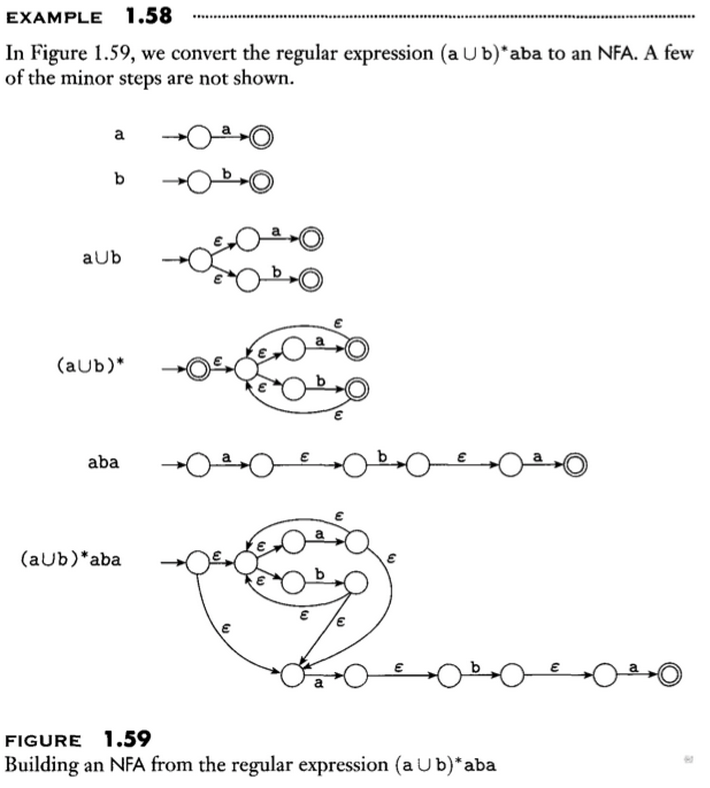
\includegraphics[scale=0.25]{regex_to_nfa.png}
  \end{center}

  \subsection{NFA $\rightarrow$ Regex}

  Remove states one at a time, maintain equivalence, until we get two states with one regex transition.
  \begin{itemize}
    \item Add new start state with an $\epsilon$ arc to old start state
    \item Add new single ccpet state, connected with $\epsilon$ arcs from old accept states
    \item No arcs into start state or out of accept state
    \item All other arcs present (with $\emptyset$ label if necessary)
  \end{itemize}


  \subsection{DFA $\rightarrow$ Regex}

  This is aided by a {\bf generalized nondeterministic finite automaton} defined as the 5-tuple $(Q, \Sigma, \delta, q_{start}, q_{accept})$. $Q$ is the finite set of states, $\Sigma$ is the input alphabet, $delta: (Q - \{q_{accept}\}) x (Q - \{q_{start}\}) \rightarrow R$ is the transition function.

  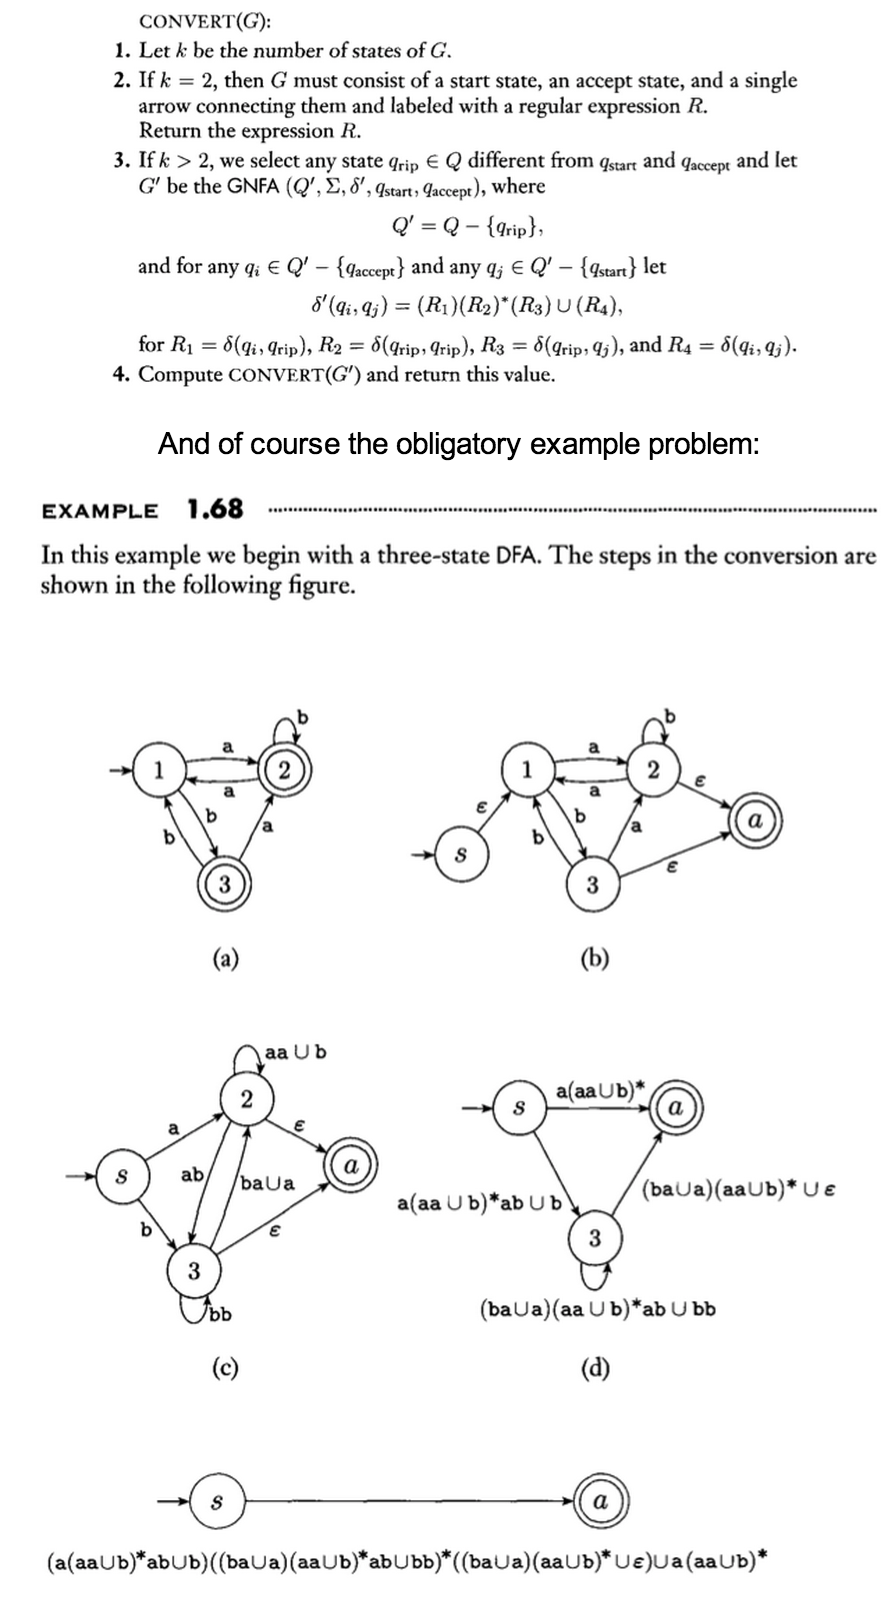
\includegraphics[scale=0.25]{dfa_to_regex.png}

  \section{Nonregular Languages}

  Any language that can not be determined in a finite amount of states on a DFA or NFA is nonregular. Good examples are languages that require the knowledge of a previous count to prove them, such as a language that has some number of $0$ followed by the same number of $1$s.

  \subsection{Pumping Lemma}

  The pumping lemma is a simple proof to show that a language is not regular, meaning a FSM can not be built for it. The canonical example is the language $(a^n)(b^n)$. It is trivial to build a FSM for some examples:

  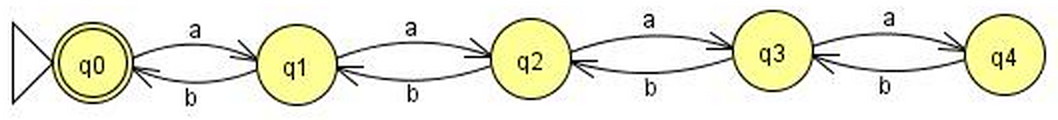
\includegraphics[scale=0.25]{simple_pumping_fsm.png}

  Such an FSM will work all the way up to $n = 4$, but the language does not constrain $n$. No matter how many states are added to the FSM, there will be an input where $n$ is the number of states plus $1$, and the machine will fail. Therefore, we must add a loop in the FSM to keep the number of states finite, as such:

  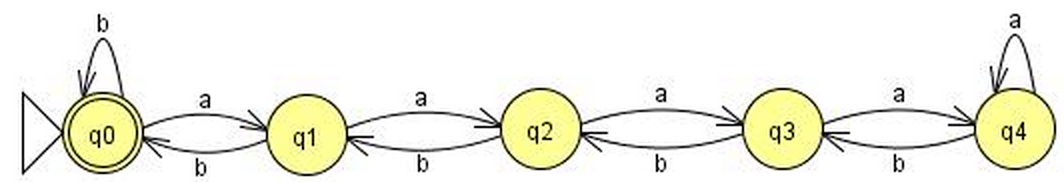
\includegraphics[scale=0.25]{loop_pumping_fsm.png}

  This will work. However, after the first $4$ $a$s, the machine loses count of how many have bene input because it stays in the same state. Therefore, this erroneously accepts the string $aaaa(a^*)bbbb$. We can say that $(a^*)$ can be pumped. The fact that the FSM is finite and $n$ is not bounded guarantees that any machine which accepts all strings in the language must have this property -- the machine must loop at some point, and when it loops, the language can be pumped. Therefore, no FSM can be built for this language, thus it is not regular.

  Mathematically, let $L$ be a regular language. Then there exists an integer $p >= 1$ depending only on $L$ such that every string $w$ in $L$ of length $>= p$ can be written as $w = wyx$, i.e. $w$ can be divided into 3 substrings, such that:

  \begin{itemize}
    \item $|y| >= 1$
    \item $xy <= p$
    \item $\forall i >= 0, xy^iz \in L$
  \end{itemize}

  $y$ is the substring that can be {\bf pumped} (removed or repeated any number of times, and the resulting string is always in $L$). $(1)$ means the loop $y$ to be pumped must be of length at least $1$, $(2)$ means the loop must occur within the first $p$ characters. $|x|$ must be smaller than $p$ by $(1)$ and $(2)$; apart from that there is no restriction on $x$ and $z$.

  In other words, for any regular language $L$, any sufficiently long word $w \in L$ can be split into $3$ parts, $w = xyz$, such that all the strings $xy^kz$ for $k >= 0$ are also in $L$.

  \subsubsection{Game}

  Consider $ADD = \{$``$a + b = c$"$\}$, e.g. $2 + 3 = 5 \in ADD$, but $2 + 3 = 6 \notin ADD$.

  Can a $17$-state DFA $M$ recognize this language? {\bf No}. Consider $1, 2, 3, ..., 18$ as the value for $a$. Two different numbers, e.g. $2$ and $5$, get $M$ to the same state. Then $2 + 1 = 3, 5 + 1 = 3$ take $M$ to the same state. {\bf CONTRADICTION}.

  Paula wants to prove that a language is regular; skeptical Victor wants to verify.

  Paula: ``This 17-state $M$ recognizes $ADD$\\
  Victor: ``Oh, really? What if we start with $1, 2, ..., 18$?\\
  {\bf Victor wins; $ADD$ is not regular}

  - - - - - - - - - - - - 

  Show $A = \{ww: w \in \Sigma^*\}$ is not regular.

  Paula: $p$\\
  Victor: $w = 10^{p+1}$\\
  Paula: $ww = xyz$ with $|y| > 0, |xy| <= p$\\
  Victor: $i = 0$\\
  $y \in 0^+$ has exactly one $1$. $x = $``1", $y =$ ``00", $z =$ ``0010000" $\rightarrow w =$ ``1000010000". Alternatively, $w = 1000|010|000$. So $xz$ has unequal $0$ fields or an odd number of $1$s. $xz \notin A \rightarrow$ contradiction.

  \subsubsection{General for Regular Languages}

  If a language $L$ is regular, then there exists a number $p >= 1$ such that every string $uwv \in L$ with $|w| >= p$ can be written in the form $uwv = wxyzv$ with strings $x, y, z$ such that $|xy| <= p, |y| >= 1$, and $uxy^izv \in L \forall i >= 0$.

  \subsubsection{Converse}

  The converse of the pumping lemma is not true; a language that satisfies the conditions may still be non-regular. Both the original and general versions of the lemma necessary {\bf but not sufficient condition} for the language to be regular.

  \section{Turing Machines}

  Hypothetical devices that manipulate symbols on a strop of tape according to some table of rules. Consists of:

  \begin{itemize}
    \item A {\bf tape} divided into cells, one next to the other. Each cell contains a symbol from some finite alphabet. The alphabet contains some special blank symbol and one or more other symbols. The tape is assumed to be arbitrarily extendable to the left and right. Cells that have no content are assumed to be filled with the blank symbol.
    \item A {\bf head} that can read and write symbols on the tape and move the tape left and right one cell at a time.
    \item An {\bf action table or transition function} of instructions that, given the state the machine is currently in and the current symbol being read from the tape, tells the machine to do the folliwing in sequence:

      \begin{itemize}
        \item Either erase or write a symbol, and then
        \item Move the head, and then
        \item Assume the same or a new state as prescribed
      \end{itemize}
  \end{itemize}

  Note that every part of the machine and its actions is finite, discrete and distinguishable.

  \subsection{Formal Definition}

  7-tuple $M = (Q, \Gamma, \beta, \Sigma, \delta, q_0, F)$, where:

  \begin{itemize}
    \item $Q$ is a finite, non-empty set of states
    \item $\Gamma$ is a finite, non-empty set of the tape alphabet/symbols
    \item $\beta \in \Gamma$ is the blank symbol (the only symbol allowed to occur on the table indefinitely often at any step during the computation)
    \item $\Sigma \subseteq (\Gamma - \{\beta\})$ is the set of input symbols
    \item $q_0 \in Q$ is the initial state
    \item $F \subseteq Q$ is the set of final/accepting states
    \item $\delta: (Q - \{F x \Gamma\}) \rightarrow Q x \Gamma x \{L, R\}$ is a partial function called the transition function, where $L$ is left shift, $R$ is right shift, $N$ is no shift.
  \end{itemize}

  \subsubsection{3-State Busy Beaver}

  A turing machine that attains the maximum number of steps performed or number of nonblank symbols finally on the tape among all Turing machines of a certain class.

  \begin{itemize}
    \item $Q = \{A, B, C, HALT\}$
    \item $\Gamma = \{0, 1\}$
    \item $\beta = 0$ ("blank")
    \item $\Sigma = \{1\}$
    \item $q_0 = A$ (initial state)
    \item $F = \{HALT\}$
    \item $\delta$ is given on attached page
  \end{itemize}

  \section{Decidable Languages}

  A decidable language is:

  \begin{itemize}
    \item A recursive subset in the set of all possible words over the alphabet of the language
    \item A formal language for which there exists a Turing machine which will, when presented with any finite input string, halt and accept if the string is in the language, and halt and reject otherwise. The Turing machine always halts; it is known as a decider and is said to decide the language.
  \end{itemize}

  \subsection{Decider}

  A decider is a machine that halts for every input. Also known as a total turing machine. $L(M)$ is decidable.

  \subsection{Closure Properties}

  Decidable languages are closed under the following operations (if $L$ and $P$ are two decidable languages, then the following are also decidable):

  \begin{itemize}
    \item Kleene star $L^*$
    \item Concatenation $L . P$
    \item Union $L \cup P$
    \item Intersection $L \cap P$
    \item Complement $\bar{L}$
    \item Set difference $L - P$ (can be expressed in terms of intersection and complement)
  \end{itemize}

  \subsection{Decidability}

  Let $A_{DFA} = \{<B, w> | B$ is a DFA that accepts input string $w \}$

  \begin{itemize}
    \item Need to present a Turing machine $M$ that decides $A_{DFA}$
    \item $M = $``On input $<B, w>$, where $B$ is a DFA and $w$ is a string:
      \begin{itemize}
        \item Simulate $B$ on input $w$
        \item If the simulation ends in an accept state, accept. Otherwise, reject
      \end{itemize}
    \item When $M$ receives its input, it checks whether the input is actually a DFA and string. If not, reject.
    \item $M$ then carries out the simulation, keeping track of $B$'s state and position on its tape
    \item When $M$ finishes processing the last symbol of $w$, it accepts if $B$ is in an accepting state; rejects otherwise.
  \end{itemize}

  \subsection{Undecidable Languages}

  Assume that $A_{TM} = \{<M, w>: M(w)$ enters ``accept"$\}$ is undecidable. The following are undecidable:
  \begin{itemize}
    \item $\{<M, w>: M(w)$ enters state $q_5\}$
    \item $\{<M, w>: M(w)$ prints $5\}$
    \item $\{<M, w>: M(w)$ enumerates $0^n1^n\}$
    \item $\{<M>: M()$ enumerates $0^n1^n\}$
    \item $\{<M>: M()$ enumerates a regular language$\}$
    \item $\{<M>:$ For $M$ as an enumerator, $L(M)$ is regular$\}$
    \item $\{<M>:$ For $M$ as a recognizer, $L(M)$ is regular$\}$
    \item $\{<M>:$ For $M$ as a recognizer, $L(M)$ is ...$\}$
  \end{itemize}

  \subsubsection{Halting Problem}

  $A_{TM} = \{<M, w> | M$ is a TM and $M$ accepts $w\}$\\
  Theorem: $A_{TM}$ is undecidable.\\
  Proof:

  \begin{itemize}
    \item Assume $A_{TM}$ is decidable. Suppose $H$ is a decider for $A_{TM}$: $H(<M, w>) = \{$accept if $M$ accepts $w$; reject otherwise$\}$
    \item Construct a new TM $D$ that calls $H$ to determine what $M$ does when $M$ is its own input. $D = $``On input $<M>$:
      \begin{itemize}
        \item Run $H$ on input $<M, <M> >$
        \item Output the opposite of what $H$ outputs
      \end{itemize}
    \item Example of $D$: $D(<M>) = \{$ accept if $M$ does not accept $<M>$, reject if $M$ accepts $<M>\}$
    \item Run $D$ with itself as input: $D(<D>) = \{ $accept if $D$ does not accept $<D>$; reject if $D$ accepts $<D>\}$
    \item No matter what $D$ does, it is forced to do the opposite $\rightarrow$ contradiction. Thus, neither $D$ nor $H$ can exist. Therefore, $A_{TM}$ is undecidable.
  \end{itemize}

  \subsection{Relationships}
  \begin{itemize}
    \item If $L$ is decidable, then $L$ is recognizabl. {\bf Given decider $D$, let $R$ simulate $D$. If $D$ is about to enter REJECT, then $R$ instead loops}
    \item The decidable languages are closed under complement. {\bf Exchange REJECT and ACCEPT states.}
    \item The recognizable languages are closed under projection. If $\{(x, y): P(x, y)\}$ is some decidable language of pairs, then $\{x : \exists y P(x, y)\}$ is recognizable. {\bf Given $R$ for the pairs language, build $R'$ to try all $y$, breadth-first, and simulate $R(x, y)$}
    \item The recognizable languages are not closed under complement, so some recognizable language is not decidable
    \item $L$ has a recognizer iff $L$ has an enumerator
    \item $L$ has a decider iff $L$ has an enumerator that outputs {\bf in lexicographic order}
  \end{itemize}

  \subsection{Equivalencies}
  \begin{itemize}
    \item If $L$ has a recognizer $R$, then a simulating enumerator $E$ tries all strings $w = \epsilon, 0, 1, 00, ...$ breadth-first and prints $w$ if $R(w)$ accepts. Then $L(R) \subseteq L(E)$, $L(E) \subseteq L(R)$
    \item If $L$ has an enumerator $E$, then a simulating recognizer $R$ on input $w$ runs $E$. $R$ accepts if $R$ sees that $E$ prints $w$
    \item If $L$ has a decider $D$, then a simulating emulator $E$ tries all strings $w = \epsilon, 0, 1, 00, ...$ depth-first
    \item If $L$ is finite, $L$ has a decider. Otherwise, if $L$ has a sorted-order enumerator $E$, then a simulating decider $D$ on winput $w$ runs $E$. $D$ accepts $w$ if $D$ sees that $E$ pritns $w$, and $D$ rejects $w$ if $D$ sees that $E$ prints anything after $w$
    \item If $L$ is recognizable and $\bar{L}$ is recognizable, then $L$ is decidable
    \item Some language is neither recognizable nor co-recognizable
    \item If $A_{TM}$ were co-recognizable, $A_{TM}$ would be decidable. On input $<M, w>$, interleave recognizers for $A_{TM}$ and $\overline{A_{TM}}$. When one of the recognizers halts, decide $<M, w> \in A_{TM}$. So $\overline{A_{TM}}$ is not recognizable.
    \item Similarly, if $L$ is recognizable and co-recognizable, then $L$ is decidable.
  \end{itemize}


  \subsection{Recognizers}

  Recognizers either reach {\bf accept} or loop forever. $L(M) = \{w : M(w)$ reaches ACCEPT$\}$ is recognizable.

  \subsection{Enumerators}

  An enumerator is a variant of a TM with an attached printer; used as an output device to print strings. Every time the TM wants to add a string to the list of recognized strings it sends it to the printer.\\
  An enumerator starts with a blank input tape. If it does not halt, it may print an infinite list of strings.\\
  The language recognized by the enumerator is the collection of strings that it eventually prints out. These strings may be generated in any order, possibly with repetitions.

  {\bf Theorem:} A language $A$ is Turing-recognizable iff some enumerator enumerates it.

  {\bf if:} If $A$ is recognizable it means that there is some TM $M$ that recognizes $A$. Then we can construct an enumerator $E$ for $A$. For this, consider $s_1, s_2, ...$, the list of all possible strings in $\Sigma^*$, where $\Sigma$ is the alphabet of $M$.

  $E =$ ``Ignore the input.
  \begin{itemize}
    \item Repeat for $i = 1, 2, 3, ...$
    \item Run $M$ for $i$ steps on each input $s_1, s_2, ..., s_i$
    \item If any computation accepts, print the corresponding $s_j$
  \end{itemize}

  Note that if $M$ accepts $s$, eventually it will appear on the list generated by $E$. It will appear infinitely many times because $M$ runs from the beginning on each string for each repetition of step $1$ -- it appears that it runs in parallel on all possible input strings.

  {\bf only if:} If we have an enumerator $E$ that enumerates a language $A$ then a TM $M$ recognizes $A$. $M$ operates on input $w$:
  \begin{itemize}
    \item Run $E$ on $w$. Every time $E$ outputs a string, compare it with $w$
    \item If $W$ ever appears in the output of $E$, accept.
  \end{itemize}

  Clearly, $M$ accepts those strings that appear on $E$'s list.

  \subsection{Double Indefinite Tape}

  A Turing machine with double indefinite tape has indefinite tape to the left and right. Assume that the tape is initially filled with blanks except for the portio that contains the input. Show that a TM $D$ with double infinite tape can simulate an ordinary TM $M$ and $M$ can simulate a TM $D$ with double infinite tape.

  \subsubsection{Simulating $M$ by $D$}

  A TM $D$ with double infinite tape can simulate $M$ by marking the left-hand side of the input to detect and prevent the head from moving off that end.

  \subsubsection{Simulating $D$ by $M$}

  First, we show how to simulate $D$ with a 2-tape TM $M$
  \begin{itemize}
    \item The first tape of $M$ is written with the input string; second tape is blank
    \item Cut the tape pf the double infinite tape TM into two parts at the starting cell of the input string
    \item The portion with the input string and all blank spaces to its right appears on the first tape of the 2-tape TM. The other portion appears on the second tape in reverse order.
  \end{itemize}

  \subsection{Multi-Tape Turing Machines}

  {\bf Theorem:} Every multitape Turing machine has an equivalent single tape Turing machine.\\
  {\bf Proof:} We show how to convert a multitape TM $M$ into a single tape TM $S$. Assume that $M$ has $k$ tapes. $S$ will simulate the effect of $k$ tapes by storing their information on its single tape. $S$ uses a symbol ``\#" as a delimeter to separate the contents of the tapes, and keeps track of the locations of the heads by marking the symbols where the heads should be with a dot.\\
  $S = $``On input $w = w_1w_2...w_n$
  \begin{itemize}
    \item Put $S(tape)$ in the format that represents $M(tapes)$, described above
    \item Scan the tape from the first ``\#" (representing the left-hand end) to the $(k+1)$st ``\#" (right-hand end) to determine the symbols under the virtual heads. Then $S$ makes a second pass to update it according to $M$'s $\delta$ function
    \item If $S$ moves one of the virtual heads to the right of a ``\#", $M$ has moved on the corresponding tape to unread blank contents. So $S$ shifts the tape contents from this cell until the rightmost ``\#" and writes a blank value on the freed tape cell. It continues the simualtion.
  \end{itemize}

  \section{Rice's Theory}

  A property of recognizable languages is itself a recognizable language. Because of this, ``regularity" is a property. If language $L$ has a nontrivial property $P$, such that $\{<M>: L(M) \in P\}$, $L$ is not decidable. This indicates that {\bf if a language has some nontrivial property, it is not decidable}.

  Note that the theorem does not stipulate whether a language is {\bf recognizable}

  \subsection{Non-Trivial Property}

  A {\bf property} is a set of recognizable languages, e.g. regularity, ``two $a$s", etc.\\
  A {\bf non-trivial property} $P$ is a language which contains and avoids at least one recognizable language. Simply, $P$ if any property which requires more computing capability than can effectively be used, thus can not be decided.

%\section{Post's Correspondence}

%TODO

%\section{Godel's Incompleteness}

%TODO

  \section{Countability}

  A set is considered countable if it either has a finite number of elements or it has the same size as the set of natural numbers ($\{0, 1, 2, 3, ...\}$). {\bf The real numbers are uncountable}

  \section{Misc Theorems}

  \begin{itemize}
    \item The class of regular languages is closed under the union operation
    \item The class of regular languages is closed under the concatenation operation
    \item The class of regular languages is closed under the star operation
    \item Every nondeterministic finite automaton has an equivalent deterministic finite automaton
    \item A language is regular iff some nondeterministic finite automaton recognizes it
    \item A language is regular iff some regular expression describes it
    \item If a language is described by a regular expression, then it is regular
    \item Every multitape Turing machine has an equivalent single tape turing machine
    \item A language is Turing-recognizable iff some multitape Turing machine recognizes it
    \item A language is Turing-recognizable iff some enumerator enumerates it
    \item Regular expressions, NFAs, and DFAs are decidable
    \item Every context-free language is decidable
    \item The set of real numbers is uncountable
    \item Some languages are not Turing-recognizable
    \item A language is decidable iff it is Turing-recognizable and co-Turing recognizable
    \item Regular languages are undecidable
    \item If $M$ is a linear bounded automaton (Turing machine where tape head states inside of the input) where $L(M) = \emptyset$, then the machine $M$ is undecidable
    \item If $G$ is a context-free grammar and $L(G) = \Sigma^*$, then the machine $G$ is undecidable
  \end{itemize}

  \section{Mapping Reducability}

  Mapping a language $A$ onto language $B$ is easily solvable. Since we mapped $A$ onto it, we can use the solver for $B$ to show that $A$ is solvable. Let's say you can check if a string is in $B$ or not. You want to determine whether a string $x \in A$. {\bf Map} $x$ by $f$, yielding $f(x)$, then check if it is in $B$. $f$ is a mapping reduction if $(x \in A) \leftrightarrow (f(x) \in B)$.

  \subsection{Comparable Function}
  A function $f: \Sigma^* \rightarrow \Sigma^*$ is a computable function if $\exists$ some TM $M$ that, on every input $w$, halts with just $f(w)$ on the tape.

  \subsection{Reduction}
  Language $A$ is {\bf mapping reducable} to language $B$, written as $A <=_m B$, if there is a computable function $f: \Sigma^* \rightarrow \Sigma^*$, where $\forall w, w \in A \leftrightarrow f(w) \in B$. The function $f$ is called the {\bf reduction} of $A$ to $B$.

  \section{Turing Reducability}

  Turing reductions can {\bf NOT} be used to show that a problem is $NP-$complete.

  \subsection{Oracle}
  A device for language $B$ that tells whether any string $w$ is a member of $B$. It doesn't matter how it does this (``magic" is valid); can be applied to languages that aren't decidable

  \subsection{Oracle Turing Machine}
  A Turing Machine that has the added capability of querying an oracle, denoted $M^B$

  \subsection{Turing Reducible}
  Language $A$ is {\bf Turing reducible} to language $B$, written $A <=_T B$, if $A$ is decidable relative to $B$. Turing reductions are stronger than mapping reductions, in the sense that they are more flexible. However, this flexibility comes at a cost -- for example, one can not use a Turing reduction to show that a problem is {\bf NP-hard}.

  \section{Complexity}

  \subsection{Time Complexity}
  For deterministic TMs, the time complexity $f(n)$ is the maximum number of steps it takes on an input of length $n$.

  \subsection{Big-O}
  The asymptotic upper bound of a function -- formally $f(n) = O(g(n)) \rightarrow g(n)$ is the upper bound. Big-O can appear in the exponent and behaves similarly, as in $f(n) = 2^{O(n)}$, which is like saying that the function is bound by some power of $2$ (e.g. $((2^c)^n)$). $\exists k: f(x) <= k \times g(x)$. If $\lim_{x \rightarrow \infty} |\frac{f(x)}{g(x)}| < \infty$, then $f(x) = O(g(x))$.

  \subsubsection{Polynomial Bounds}
  $n^c$, where $c > 0$

  \subsubsection{Exponential Bounds}
  $c^n$

  \section{Small-O}
  Similar to Big-O, but a strict upper bound (``it WILL take less time than this"). $\forall k: f(x) < k \times g(x)$. If $lim_{x \rightarrow \infty}|\frac{f(x)}{g(x)}| = 0, f(x) = o(g(x))$.

  $TIME(t(n))$ is the collection of all languages that are decidable by an $O(t(n))$ TM.

  \subsection{$P$, $NP$}

  \subsubsection{$P$}
  The class of problems that are solvable in a polynomial time regardless of computation model ($O(n^{O(1)}$). If the runtime is polynomial, then the size of input, output and sapce must also be polynomial with the lenght of the input.

  P is not closed under projection, e.g. the verification of $HAMPATH \in P$, but $HAMPATH$ itself (the projection of $HAMPATH$ verification) is in $NP$.

  \subsection{$NP$}
  $P$ is a subset of $NP$, which is the class of languages that have a polynomial-time verifier.

  \subsection{$P$ vs $NP$}
  {\bf $P$} is the class of languages for which membership can be {\em decided} quickly. {\bf $NP$} is the class of languages for which membership can be {\em verified} quickly.

  {\bf $NTIME(t(n))$} is a collection of languages decided by an $O(t(n))$ time non-deterministic Turing machine. $NP$ is the union of all languages in $NTIME(n^k)$.

  \section{TQBF}
  True Quantified Boolean Formula -- a fully qualified formula. Written as $\Phi \forall x \exists y [(x \vee y) \wedge (\neg x \vee \neg y)]$. If such a formula evaluates to true, then it is in TQBF. Also known as Quantified SAT (QSAT).

  \subsection{FORMULA-GAME}
  A game with two players $A$ and $E$. Each player selects a value of a variable quantified either the $\forall$s if the player is $A$, or $\exists$s if player $E$, based on the order of the quantifiers. In the end, if the formula is $TRUE$ player $E$ wins, else player $A$ wins.

  Consider this as Peggy vs. Victor. Peggy takes existential qualifiers, Victor takes universal ones. They don't have to alternate turns -- the order is specified by the order of quantifiers in the expressions.

  \section{Problems}

  \subsection{SAT}

  Boolean satisfiability problem -- the problem of determining if there exists an interpretation which satisfies a given formula -- in other words, establishes if the variables of a given boolean formula can be assigned in such a way as to make the formula evaluate to TRUE.
  
      \subsubsection{Literal}
      A literal is either a variable or the negation of a variable
      \subsubsection{Clause}
      A clause is a disjunction of literals
      \subsubsection{NP-Completeness}
      SAT is NP-complete.
      \subsubsection{3-Satisfiability}
      Special case of $k-$satisfiability when each clause contains exactly $k = 3$ literals. For example, $E = (x_1 \vee \neg x_2 \vee \neg x_3) \wedge (x_1 \vee x_2 \vee x_4)$. E has two clauses, four variables, and $k = 3$. This is NP-complete, and is used as a starting point to prove that other problems are also NP-hard via a polynomial-time reduction from 3-SAT to the other problem.

  \subsection{HAMPATH}
  A directed graph in which all vertices can be hit just once. Polynomially verifiable, but is not solvable in polynomial time.

  \subsection{UNHAMPATH}
  An undirected graph in which all vertices can be hit just once. Polynomially verifiable, but not solvable in polynomial time.

  \subsection{CLIQUE}
  A clique is a subgraph wherein every two nodes are conected by an edge; a $k-$clique is a clique that contains $k$ nodes.

  \subsubsection{MAXCLIQUE}

  TODO

  MAXCLIQUE is $NP-$hard.

  \subsubsection{Decision Version}

  TODO

  Is there a $k$-clique in a given graph G?

  NP-Complete

  \subsection{SUBSET-SUM}
  A problem concerning integer arithmetic, where we have numbers $x_1, ..., x_k$ and a target number $t$. We want to determine whether the collection contains a subcollection that adds up to $t$. This problem is $NP-$complete.

  \subsection{3SAT}
  A special instance of the satisfiability problem, written in {\bf 3CNF}-form: $\Phi = (x_1 \vee x_2 \vee x_3) \wedge (x_4 \vee x_5 \vee x_6) ...$. TODO

  \subsection{VERTEX-COVER}
  For an undirected graph $G$, a vertex cover is a subset of nodes where every edge of $G$ touches one of those nodes.

  \subsection{3COL}

  Graph 3-colorability. NP-complete.

  TODO: More

  \subsection{TODO: MORE}

  \section{NP-Completeness}
  There are certain problems $\in NP$ whose complexity is related to the entire class of $NP$, so if one polynomial time algorithm is found, then all of $NP$ is solvable in polynomial time.

  \subsection{Formal Definition}
  A language $B$ is NP-complete if both $B \in NP$ and every $A$ in $NP$ is polynomial-time reducible to $B$. {\bf The second condition indicates that $B$ is $NP-$hard}

  \subsection{Cook-Levin}
  $SAT \in P iff P = NP$ -- $SAT$ is $NP-$complete.

  \section{Polynomial-Time Reduction}
  Language $A$ is {\bf polynomial time mapping reducible} to language $B$, written $a <=_p B$, if there is a polynomial-time computable function $f: \Sigma^* \rightarrow \Sigma^*$ where $\forall w, w \in A \leftrightarrow f(w) \in B$. The function $f$ is called the {\bf polynomial time reduction} of $A$ to $B$.
  
  These reductions are computable by a deterministic TM in polynomial time. They are powerful enough to perform many transformations between important problems. These reductions are not appropriate for use in class $P$, because any problem in $P$ can be polynomial-time reduced to almost any other problem in $P$.

  \section{Space Complexity}
  Whereas in the last section we were dealing with time, now we consider space as the number of cells the TM uses.

  TODO: FIGURE 8.7

  \subsection{SPACE(f(n))}
  A language decided by an $O(f(n))$-space deterministic TM.

  \subsection{NSPACE(f(n))}
  A language decided by an $O(f(n))$-space nondeterministic TM

  \subsection{PSPACE}
  The class of languages that are decidable in polynomial space on a deterministic TM. {\bf $PSPACE = NPSPACE$ via Savitch's Theorem}.

  \subsubsection{PSPACE Completeness}
  A language $B$ is PSPACE-complete if $B$ is in PSPACE and $\forall A \in PSPACE, A$ is polynomial time reducible to $B$. If only the second is satisfied, then it is $PSPACE-hard$

  \section{Approximation Algorithms}
  While we usually look for a best {\bf optimal} solution, an approximately optimal solution will usually suffice. Approximation algorithms are designed to find this.

  \subsection{2-approx for minVC}
  Let $G$ be a graph with the set of edges $E$.

  C = $\emptyset$ (vertex cover approximate graph).

  While there is some edge $e = \{u, v\} \in E$,

  \hspace{10px} $C \leftarrow C \cup \{u, v\}$

  \hspace{10px} $G \leftarrow G - \{u, v\}$

  Let $C^*$ be the optimal (minimal) vertex cover. Then $C^* <= C <= 2C^*$.

  The first indented step above adds vertices $u$ and $v$ to graph $C$, and the second removes $u, v$ and all adjacent edges from $G$.

  \section{Zero Knowledge Proofs}
  A zero knowledge proof is an interaction between Peggy (prover) and Victor (verifier) where P tries to convince V that a given statement is true without conveying any information besides the truth value of the statement.

  Such a proof must have:

  \begin{itemize}
    \item {\bf Completeness} - if P can solve the problem, P can convince V to accept with a high probability.
    \item {\bf Soundness} - if P cannot solve the problem there is a very low probabiliyt of P convincing V to accept
    \item {\bf Zero knowledge transfer} - The prover does not give any new information to the verifier
  \end{itemize}

  Such proofs can be simulated, but cannot be relayed to outsiders. They also are not deterministic and are probabilistic proofs, not mathematical.

  \subsection{ZKP for Graph Non-Isomorphism}

  TODO: Define isomorphism

  P is trying to convince V that graphs $G_1, G_2$ are not isomorphic.

  On input $G_1 = (V, E_1), G_2 = (V, E_2)$ 
  \begin{itemize}
    \item V picks random $b \in \{1, 2\}$ and permutation $\pi: V \rightarrow V$; sends $G = \pi(G_b)$ to P
    \item P finds $a \in \{1, 2\}$ such that $G_a$ and $G$ are isomorphic; sends $a$ to $V$.
    \item V checks that $a == b$, and accepts if so
  \end{itemize}

  If $G_1, G_2$ are not isomorphic, P can always determine which one V started from, so V accepts with probability 1.

  If $G_1, G_2$ are isomorphic, P cannot determine which one $V$ started from, so $V$ accepts with probability $w^{-k}$, with $k$ being the number of repetitions.

  Because V already knows the answer, no transfer of knowledge occurs.

  TODO: What happens if someone behaves predictably instead of randomly?

  \subsection{Color-Blindness}

  Imagine your friend is color-blind. You have two balls: one red, one green, but otherwise identical. You want to prove to him that they are differently colored, without having him learn which is red and which is green.

  Give the two balls to him so one is in each hand. Don't tell him which is which. Have him put both hands behind his back. He will either switch the balls between his hands or leave them, with $P = 0.5$ of either event. He brings them in front of him, showing them. You now have to ``guess" whether or not they were switched. By identifying whether or not the balls were switched, using the colors, you can prove that your friend is colorblind after a number of repetitions.

  \subsection{Graph-3-Colorability}

  The public input is a graph $G(V, E)$ of $n$ vertices and $m$ edges, with $m <= n^2$. P gets as private input a function $c: V \rightarrow \{R, G< B\}$ such that $\forall (u, v) \in E, c(u) \neq c(v)$.

  P chooses a random 1-to-1 function $\Gamma: \{R, G, B\} \rightarrow \{1, 2, 3\}$. P defines $c': V \rightarrow \{1, 2, 3\}$ to be such that $\forall v \in V, c'(v) = \Gamma(c(v))$. P computes $y_1, ..., y_n$ such that $y_i$ is a commitment to $c'(v_i)$, where $v_i$ is the $i^{th}$ vertex. P then sends $y_1, ..., y_n$ to V.

  V chooses a random edge $(v_i, v_j) \leftarrow_R E$ and sends $(v_i, v_j)$ to P.

  P sends $r_i, r_j \in \{0, 1\}^n$ and $x_i, x_j \in \{1, 2, 3\}$ such that $y_i = C(x_i, r_i); y_j = C(x_j, r_j)$. These two are considered the openings.

  V accepts iff the openings are valid, $x_i, x_j \in \{1, 2, 3\}$, and $x_i \neq x_j$.

  To show soundness, show that if $G$ is not $3-$colorable, then V will reject with probability of at least $1 - \frac{1}{m}$, where $m$ is the number of edges.

  \subsection{Sudoku}

  TODO

  \section{Theorems}

  TODO

  \section{NP-Hard Problems}

  TODO: Enumerate...

  CLIQUE, IS, VS

  \section{Definitions}

  {\bf Soundness}: A resolution is sound if it never declares satisfiable formulas unsatisfiable (``no" means no).

  {\bf Completeness}: A resolution is complete if all unsatisfiable formulas are declared unsatisfiable.

  TODO: List of reductions!

  \section{Homework Problems}

  \subsection{HW6}

  {\bf Show how to compute $a^b mod p$, where $p$ is prime, in polynomial time in the length of the input $(a, b, p)$}

  A straightforward approach is to multiply $a$ by itself $b$
  times, for a total of $b-1$ multiplications, then take the result mod
  $p$.  This fails on two counts:  The number of multiplications is
  approximately $b$, which is exponential in the {\em length} of $b$.
  And, no matter how we ended up with $a^b$, the length of $a^b$ is
  $b\cdot|a|$, which is too long to handle (read, write, etc.)

  The solution is to do repeated squaring and reduce mod $p$ as we go.
  As for the hint, I meant to write ``first try $b$ a power of 2.''  If
  $b=32$, then $a^b$ is $((((a^2)^2)^2)^2)^2$.  This involves just 5
  multiplications.  We need to reduce mod $p$ as we go, so we get
  $(\cdots(a^2\bmod p)^2\bmod p\cdots)$.  We end up doing the
  transformation $x\to x^2\bmod p$ 5 times, and each transformation
  takes time polynomial in the length of the operands and produces
  output that is of length at most $|p|$.  In general, if $b=2^\beta$,
  we perform the transformation $\beta=|b|$ times.

  Now consider general $b$.  Henceforth, all arithmetic is considered to
  be modulo $p$ and we reduce modulo $p$ where ever possible; we focus
  on the repeated squaring.  First compute $a,a^2,a^4,a^8,a^{16},\ldots$
  by repeated squaring, as above.  Then multiply together $a^{2^k}$ if
  $1\cdot 2^k$ appears in the binary representation of $b$.  As an
  example, if $b=13=1101_2$, then we compute $a^8\cdot a^4\cdot a$.  The
  number of $a^{2^k}$ that we compute is $O(\log b)$, as desired, and
  the number of multiplications we need to combine the factors of
  $a^{2^k}$ is also $O(\log(b))$.

  One could also state this inductively in $b$.  As a base case,
  $a^0=1$.  If $b>0$ and even, then
  $a^b=\left(a^{\frac b2}\right)^2$.  If $b>0$ and odd, then
  $a^b=a\cdot a^{b-1}$.  To analyze this, let $M(b)$ denote the number
  of multiplications needed to form $a^b$.  We have
  \[
    M(b)=
    \left\{
      \begin{array}{ll}
        1+M(b-1); & \mbox{$b>0$ and $b$ odd}\\
        1+M(b/2); & \mbox{$b>0$ and $b$ even}\\
               0; & \mbox{$b=0$}
      \end{array}
      \right.
    \]
    Note that, if $b$ is odd, we are not reducing $b$ by much immediately,
    though $b$ is reduced on the {\em next} step.  That is, if $b$ is odd
    and $b>1$, we get $M(b)=1+M(b-1)=2+M((b-1)/2)\le 2+M(b/2)$.  Also, if
    $b$ is even, we get $M(b)=1+M(b/2)\le2+M(b/2)$.  Here we should be
    able to see that $M(b)\le 2\lg b$, but we proceed formally a little
    further.  We have $M(1)\le 2$ and
    let's avoid $b=0$ to avoid taking a log of zero.  Then we can solve
    exactly.  The inductive hypothesis is that if $2^{k-1}<b\le 2^k$, then
    $M(b)\le 2+k$.  True if $k=0$ (and $b=1$).  If it's true for all $b\le
    2^k$ and we have $2^k<b\le 2^{k+1}$, then
    \[M(b)\le 2+M(b/2)\le2+(2+\lg(b/2))\le 2+(k+1).\]

    The instructions accidentally asked you to consider $p$ a power of 2,
    say, $p=2^\pi$.  Taking $x\bmod p$ amounts to taking the $\pi$ least
    significant bits of $x$.  This can be done in time linear in $|x|$ and
    is straightforward.  For general $p$, you can do a long division with
    remainder of $x$ divided by $p$.  Assuming for simplicity that
    $|x|=|p|=n$, there will be $O(n^2)$ symbols written down in the long
    division and each symbol will take $O(1)$ time to compute.

    {\bf Give a reduction from $3SAT$ to $G3C$ (graph 3-colorability), thereby showing that $G3C$ is $NP-$hard}

    Consider the following graph:

    \begin{center}
      `\resizebox{3cm}{!}{
        \begin{picture}(160,100)(-150,-20)

          \put(-200,20){
            \put(0,0){\circle{15}}

            \put(0,40){\circle{15}}

            \put(30,20){\circle{15}}

            \put(0,8){\line(0,1){25}}

            \put(7,3){\line(3,2){17}}
            \put(7,37){\line(3,-2){17}}

            {
              \put(0,40){\makebox(0,0){$T$}}
              \put(30,20){\makebox(0,0){$G$}}
              \put(0,0){\makebox(0,0){$F$}}
            }

            {
              \put(70, 50){\circle{15}}
              \put(80, 60){\makebox(0,0){$\mathbf{A}$}}

              \put(70, 20){\circle{15}}
              \put(80, 30){\makebox(0,0){$\mathbf{B}$}}

              \put(70, -10){\circle{15}}
              \put(80,   0){\makebox(0,0){$\mathbf{C}$}}

              \put(62,48){\line(-1,-1){25}}

              \put(62,-8){\line(-1,1){25}}

              \put(62,20){\line(-1,0){25}}

              \put(70,-40){\circle{15}}

              \put(80, -30){\makebox(0,0){$\mathbf{\lnot C}$}}

              \put(64, -35){\line(-2,3){31.7}}


            }
            {

              \put(70, -32.5){\line(0,1){15}}
            }

            {

              \put(120,-10){\circle{15}}

              \put(120,20){\circle{15}}

              \put(120,-2.5){\line(0,1){15}}

              \put(77.5, 20){\line(1,0){35}}
              \put(77.5, -10){\line(1,0){35}}

              \put(150,5){\circle{15}}
              \put(160, 15){\makebox(0,0){$\lor$}}

              \put(125,-5){\line(2,1){18}}
              \put(125,15){\line(2,-1){18}}

            }

            {
              \put(70,-10){\makebox(0,0)[c]{$F$}}
              \put(70,20){\makebox(0,0)[c]{$F$}}
            }

            {
              \put(120,-10){\makebox(0,0)[c]{$T$}}
              \put(120,20){\makebox(0,0)[c]{$G$}}

              \put(120,-2.5){\vector(0,1){15}}
              \put(120,12.5){\vector(0,-1){15}}

              \put(150,5){\makebox(0,0)[c]{$F$}}
            }

            {

              \put(77.5,50){\line(1,0){115}}

              \put(157.5,5){\line(1,0){35}}

              \put(200,50){\circle{15}}
              \put(200,5){\circle{15}}

              \put(200,12.5){\line(0,1){30}}

              \put(230,27.5){\circle{15}}

              \put(205,45){\line(3,-2){19}}
              \put(205,10){\line(3,2){19}}

              \multiput(220,30)(-8,0){27}{\line(-1,0){4}}
              \multiput(8,28)(0,-8){3}{\line(0,-1){4}}

            }

            {
              \put(70,50){\makebox(0,0)[c]{$F$}}
            }

            {
              \put(200,50){\makebox(0,0)[c]{$G$}}
              \put(200,5){\makebox(0,0)[c]{$T$}}

              \put(200,12.5){\vector(0, 1){30}}
              \put(200,42.5){\vector(0,-1){30}}
            }
          }

        \end{picture}
      }
    \end{center}

    If $A, B, C$ are all colored $F$, then all the other indicated colorings are forced. The dotted edge shows that there is no possible coloring for the rightmost vertex. On the other hand, if at least one of $A, B, C$ is colored $T$, then a 3-coloring is possible:


    \begin{center}
      `\resizebox{3cm}{!}{
        \begin{picture}(160,100)(-150,-20)

          \put(-200,20){
            \put(0,0){\circle{15}}

            \put(0,40){\circle{15}}

            \put(30,20){\circle{15}}

            \put(0,8){\line(0,1){25}}

            \put(7,3){\line(3,2){17}}
            \put(7,37){\line(3,-2){17}}

            \put(0,40){\makebox(0,0){$T$}}
            \put(30,20){\makebox(0,0){$G$}}
            \put(0,0){\makebox(0,0){$F$}}

            \put(70, 50){\circle{15}}
            \put(80, 60){\makebox(0,0){$\mathbf{A}$}}

            \put(70, 20){\circle{15}}
            \put(80, 30){\makebox(0,0){$\mathbf{B}$}}

            \put(70, -10){\circle{15}}
            \put(80,   0){\makebox(0,0){$\mathbf{C}$}}

            \put(62,48){\line(-1,-1){25}}

            \put(62,-8){\line(-1,1){25}}

            \put(62,20){\line(-1,0){25}}

            \put(70,-40){\circle{15}}

            \put(80, -30){\makebox(0,0){$\mathbf{\lnot C}$}}
            \put(70, -32.5){\line(0,1){15}}

            \put(64, -35){\line(-2,3){31.7}}

            \put(120,-10){\circle{15}}

            \put(120,20){\circle{15}}

            \put(120,-2.5){\line(0,1){15}}

            \put(77.5, 20){\line(1,0){35}}
            \put(77.5, -10){\line(1,0){35}}

            \put(150,5){\circle{15}}
            \put(160, 15){\makebox(0,0){$\lor$}}

            \put(125,-5){\line(2,1){18}}
            \put(125,15){\line(2,-1){18}}

            \put(70,20){\makebox(0,0)[c]{$T$}}

            \put(77.5,50){\line(1,0){115}}

            \put(157.5,5){\line(1,0){35}}

            \put(200,50){\circle{15}}
            \put(200,5){\circle{15}}

            \put(200,12.5){\line(0,1){30}}

            \put(230,27.5){\circle{15}}

            \put(205,45){\line(3,-2){19}}
            \put(205,10){\line(3,2){19}}

            \multiput(220,30)(-8,0){27}{\line(-1,0){4}}
            \multiput(8,28)(0,-8){3}{\line(0,-1){4}}

            {
              \put(120,-10){\makebox(0,0)[c]{$G$}}
              \put(120,20){\makebox(0,0)[c]{$F$}}

              \put(150,5){\makebox(0,0)[c]{$T$}}

%\put(70,50){\makebox(0,0)[c]{$F$}}

              \put(200,50){\makebox(0,0)[c]{$G$}}
              \put(200,5){\makebox(0,0)[c]{$F$}}
              \put(230,27.5){\makebox(0,0)[c]{$T$}}
            }
          }
        \end{picture}
      }
    \end{center}


    In general, the reduction is as follows. Make a pair of vertices for each variable labeled with the variable and its negation, and form a triangle with $G$. Each clause results in $6$ more nodes and $11$ more edges, as shown. It is straightforward to build the graph from a 3CNF $\Phi$ by making a few triangles and extra edges. Now suppose $\Phi$ has a satisfying argument $v$. Color all the literal vertices $T$ or $F$ according to $v$. In each clause gadget, pick one literal colored $T$ and color its neighbor $F$. Color the rest of the clause gadget as indicated above. Thus, if $\Phi$ is satisfiable, then the graph has a 3-coloring.

    Conversely, suppose we have a 3-coloring $\Gamma$ for the graph. We can read a truth assignment from the coloring of the literal vertices. This is sensible because exactly one of $\{x, \neg x\}$ is colored $F$ and the other is $T$.

    \subsection{HW7}
    
        \subsubsection{Sudoku to adhocSAT}
            TODO
        \subsubsection{Sudoku to 3SAT}
            TODO
        \subsubsection{Sudoku to Graph Coloring}
            TODO
        \subsubsection{Farmer, Fox, Goat and Cabbage}
            TODO
    \subsection{HW8}
        \subsubsection{Specializing TQFB}
            {\bf In class, we showed how to reduce a generic PSPACE computation to an
instance of TQBF in which all the quantifiers are in front, but the
matrix (the part after the quantifiers) is arbitrary.  We also showed
that the restriction (special case) of TQBF in which the matrix is a
3-CNF reduces to Generalized Geography.  To show that Generalized
Geography is PSPACE-hard, we need to close this gap:

Show that the restriction (special case) of TQBF in which the matrix
is a 3-CNF is PSPACE-hard, by reducing a general TQBF instance to the
special case.}

            Recall that our generic reduction of PSPACE to adhocTQBF went
something like this.  Given a generic PSPACE machine $M$, we want to
define a formula $\phi(c_1,c_2,t)$ that is true iff there is a path of
exactly $t$ steps from $M$-configuration $c_1$ to $c_2$, where we may
assume that $t$ is a power of 2.  We gave a ``middle-out'' recursive
definition:
\[\phi(c_1,c_2,t)=
\left\{
\begin{array}{ll}
\exists m\forall c_3\forall c_4\>
(c_3,c_4)=(c_1,m)\lor(c_3,c_4)=(m,c_2)\to\phi(c_3,c_4,t/2), & t > 1\\
\mbox{$c_2$ equals $c_1$ except for small changes}, & t = 1.
\end{array}
\right.
\]

Note that, in the recursive constuction of $\phi(c_3,c_4,t/2)$, at
first there will be quantifiers embedded:
\[\phi(c_1,c_2,t)=
\left\{
\begin{array}{ll}
\exists m\forall c_3\forall c_4\>
(c_3,c_4)=(c_1,m)\lor(c_3,c_4)=(m,c_2)\to\left[\exists m_1\forall
  c_5\forall c_6\ldots\right], & t > 1\\
\mbox{$c_2$ equals $c_1$ except for small changes}, & t = 1,
\end{array}
\right.
\]
but, since $m_1,c_5$, and $c_6$ don't involve $m,c_3$, or $c_4$, the
quantifiers can be passed out:
\[\phi(c_1,c_2,t)=
\left\{
\begin{array}{ll}
\exists m\forall c_3\forall c_4\>\exists m_1\forall
  c_5\forall c_6\>
(c_3,c_4)=(c_1,m)\lor(c_3,c_4)=(m,c_2)\to\left[\ldots\right], & t > 1\\
\mbox{$c_2$ equals $c_1$ except for small changes}, & t = 1,
\end{array}
\right.
\]
That is, $\alpha\to\exists x\forall y\> \beta$ is the same thing as
$\exists x\forall y\>\beta$ in this case.

So we are left with a formula with all the quantifiers in front and
some quantifier-free matrix following that.

The details of the matrix depend on the precise model of computation,
which we are {\em not} specifying.  In any case, we need to express
equality of configurations, (as in $(c_3,c_4)=(c_1,m)$, above) and
{\em near} equality of configurations (as in the base case, when we
express that $c_2$ is like $c_1$ except for a small number of
changes).  For our purposes, we assume that the matrix is some boolean
formula of size polynomial in $n$, the size of input to our generic
PSPACE computation.  Our goal is to convert this to a 3-CNF, possibly
with additional quantifiers in front.

That is, we start with a formula like $\alpha=\exists w\forall x \psi(w,x)$,
where $\psi$ is an arbitrary boolean formula, and we want to get a new
formula $\beta=\exists w\forall x\exists y\forall
z\>\upsilon(w,x,y,z)$, such that
\begin{itemize}
\item $\upsilon$ is a 3-CNF
\item $beta$ is constructed from $\alpha$ in time polynomial in $n$
  (in particular, $\upsilon$ is of polynomial size), and
\item $\beta$ is true iff $\alpha$ is true.
\end{itemize}

To do this, we regard $\psi$ as a circuit and put new boolean
variables on the wires of $\psi$.  These are all existentially
quantified.  We then express that
\begin{itemize}
\item Gate-by-gate and input-by-input, $\psi$ works correctly
\item The input wires of $\psi$ agree with the original variables
  $w,x,\ldots$
\item $\psi$'s output is true.
\end{itemize}
This is similar to what we did to convert a general SAT instance into
a 3SAT instance.
        
        \subsubsection{Traveling Salesperson}

            {\bf The Traveling Salesperson Problem, \textsc{MinTSP}, is the following
optimization problem.  Consider a complete undirected graph on $n$
vertices, with a cost on each edge.  A {\em tour} is a cycle that
visits each vertex exactly once.  The cost of a tour is the sum of the
weights over edges in the tour.  The goal is to find a tour of minimum
cost.  (Formally, the input is the number $n$ of vertices and the edge
costs, but you can think of the input as the graph with edge weights.)

In \textsc{MinMetricTSP}, we are promised that the edge weights
satisfy the triangle inequality.  That is, if $C(u,v)$ denotes the
cost associated with edge $u,v$, then we are guaranteed that
$C(u,w)\le C(u,v)+C(v,w)$.

In the Minimum Spanning Tree problem, \textsc{MST}, we are given an
edge-weighted undirected connected graph $G$, as above, and the goal
is to find a tree $T$ on $G$ that is induced (edges of $T$ are in
$G$), spans (each vertex of $G$ is in $T$), and the cost is minimum,
where the cost of $T$ is the sum of the costs of the edges in $T$.

In this homework, we will walk through a 2-approximation for
\textsc{MinMetricTSP}, using an algorithm for Minimum Spanning Tree.
Polynomial-time algorithms for \textsc{MST} exist.  You're welcome to
look this up or ask about it on Piazza, but, for this homework, you
may simply assume that the algorithms are available.

Consider the following approximation algorithm for \textsc{MinMetricTSP}.

\begin{itemize}
\item Given $G$ that satisfies the triangle inequality, find a minimum
  spanning tree, $T$.
\item Duplicate each edge in $T$, getting $T'$.
\item Find an Euler tour $C'$ of $T'$.  (An Euler tour visits each
  {\em edge} exactly once.  There is an obvious polynomial-time
  algorithm for this---try to find one.)
\item Adjust $C'$ to a tour $C$ (that visits each vertex exactly
  once), by starting at some vertex $s$ and repeatedly going to the next
  {\em unvisited} vertex in $C'$, returning to $s$ in one hop
  immediately after each vertex has been visited.
\end{itemize}

Show:
\begin{enumerate}
\item This approximation algorithm runs in polynomial time (assuming a
  polynomial-time algorithm for \textsc{MST}).
\item The algorithm produces a feasible solution, {\em i.e.}, a cycle
  that visits each vertex exactly once.
\item The approximation ratio is at most 2, {\em i.e.}, the cost of
  the cycle $C$ produced is at most twice the cost of an optimal tour.
%% \item The approximation ratio of {\em this algorithm} is at least 2,
%%   {\em i.e.}, there is some graph with edge costs satisfying the
%%   triangle-inequality, on which this algorithm produces a tour with
%%   cost at least twice optimal.
\item In any optimal tour on the {\em plane} (i.e., vertices are on
  the plane and edge costs are given by Euclidean distance), no pair
  of edges cross.
\item Assuming the undirected Hamiltonian Cycle problem is NP-hard,
  show that there is no 1000-factor approximation to the general
  \textsc{MinTSP} problem (where we do {\em not} assume that the
  triangle inequality holds for edge costs.)
\end{enumerate}

Note: The factor of 2 for this approximation algorithm for
\textsc{MinMetricTSP} can be improved to the factor $3/2$, by what is
known as Christofides's algorithm.  Many variations are studied.}

            \begin{enumerate}
\item This approximation algorithm runs in polynomial time (assuming a
  polynomial-time algorithm for \textsc{MST}).

Duplicating each edge takes time linear in the number of edges.  To
find an Euler tour of a doubled tree, trace around the tree.  The
vertices will be visited in the order of a depth-first search of the
tree:

\vspace*{2in}

There are faster things to do in practice, but, to show polynomial
time for adjusting $C'$ to $C$, it suffices to trace the Eulerian tour
and to try all vertices at every stage and (easily) see whether they
are marked as having been visited.  Then mark newly visited nodes.

\item The algorithm produces a feasible solution, {\em i.e.}, a cycle
  that visits each vertex exactly once.

\solution

This is true by construction.  The Eulerian tour $T$ visits every
vertex and so $T'$, $C'$, and $C$ visit every vertex.  (Note that $C$
visits every node because we only skip a vertex $v$ in $C'$ if $v$ had
already appeared in $C$.)  And $C$ skips already-visited vertices, so
$C$ visits each vertex exactly once.

\item The approximation ratio is at most 2, {\em i.e.}, the cost of
  the cycle $C$ produced is at most twice the cost of an optimal tour.

\solution

If we take an optimal TSP tour and remove one edge, we get a spanning
tree.  So the cost of the tour must be at least as great as the cost
of the best possible spanning tree, $T$.  The cost of $T'$ is at most
twice the cost of $T$; the cost of $T'$ is exactly the cost of $C'$.
Finally, the cost of $C$ is at most the cost of $C'$.  That is,
\[c(C)\le c(C')=c(T')\le 2c(T)\le 2c(C_*),\]
where $C_*$ is the optimal TSP tour and $c(\cdot)$ is the cost.

%% \item The approximation ratio of {\em this algorithm} is at least 2,
%%   {\em i.e.}, there is some graph with edge costs satisfying the
%%   triangle-inequality, on which this algorithm produces a tour with
%%   cost at least twice optimal.
\item In any optimal tour on the {\em plane} (i.e., vertices are on
  the plane and edge costs are given by Euclidean distance), no pair
  of edges cross.

\solution

If a tentative solution had crossed edges, we can uncross the edges
and get a better tour, as follows:

\vspace*{2in}

\item Assuming the undirected Hamiltonian Cycle problem is NP-hard,
  show that there is no 1000-factor approximation to the general
  \textsc{MinTSP} problem (where we do {\em not} assume that the
  triangle inequality holds for edge costs.)

\solution

Given an instance $G=(V,E)$ of the undirected Hamiltonian Cycle
problem, we reduce to TSP as follows.  Let $n$ be the number of
vertices in $G$.  Consider the complete graph $K$ on $n$ vertices (the
same vertices as $G$), with edge weight 0 on $(u,v)$ if $(u,v)\in E$
and edge weight 1 if $(u,v)\not\in E$.  Then there is a TSP tour with
total cost zero iff there is a Hamiltonian Cycle on the original
graph.  If there is no TSP with total cost 0, then the best TSP has
cost at least 1, which is at least 1000 times optimal.  It follows
that, if we can approximate the cost of the best TSP tour to within
the factor 1000, we could distinguish a Hamiltonian graph from a
non-Hamiltonian graph.  Finally, we note that the reduction clearly
takes polynomial time.

Note:  Instead of edge weights 0 and 1, one could use edge weights 1
and $1000n$.  Then a Hamiltonian graph leads to a TSP tour of $n$
edges, each weight 1, for a total cost of $n$, whereas a
non-Hamiltonian graph leads to a TSP of total cost at least $1000n$,
which is bigger by the factor 1000.
\end{enumerate}

  \end{multicols}

%\pagebreak

  {\bf 3-State Busy Beaver State Table}

  \begin{tabular}{|c|c|c|c|c|c|c|c|c|c|c|}
    \hline
    Tape Symbol & \multicolumn{3}{|c|}{Current State A} & \multicolumn{3}{|c|}{Current State B} & \multicolumn{3}{|c|}{Current State C} \\
                & Write Symbol & Move Tape & Next State & Write Symbol & Move Tape & Next State & Write Symbol & Move Tape & Next State\\
    \hline
    0 & 1 & R & B & 1 & L & A & 1 & L & B\\
    1 & 1 & L & C & 1 & R & B & 1 & R & {\bf HALT}\\
    \hline
  \end{tabular}
  \end{document}
